% Fonte editável de fig/fluxo_spea2_pt.pdf (Figura do ciclo do SPEA2, Cap. 2).
% Reproduz o fluxograma original, sem fonte no repositório, com duas correções:
% (i) o arquivo é completado com as soluções dominadas da união da população
% corrente com o conjunto arquivo, na ordem de F(i) (Seção 2.1, passo 3), e não
% só com as do conjunto arquivo; (ii) foi retirada a caixa "F = 0", herdada do
% fluxograma do IVF/SPEA2, em que F é o número de descendentes do módulo; no
% SPEA2 ela não tem função, e F passa a denotar só a aptidão F(i).
%
% Regenerar, a partir de thesis/masters/ (a primeira compilação baixa o TikZ;
% o build da dissertação só inclui o PDF e continua offline):
%   tectonic -o fig fig/src/fluxo_spea2_pt.tex
\documentclass[border=2pt]{standalone}
\usepackage{fontspec}
\setmainfont{texgyreheros}[
  Extension = .otf,
  UprightFont = *-regular,
  BoldFont = *-bold,
]
\usepackage{tikz}
\usetikzlibrary{arrows.meta,shapes.symbols}

\begin{document}
\fontsize{10.5}{12.6}\selectfont
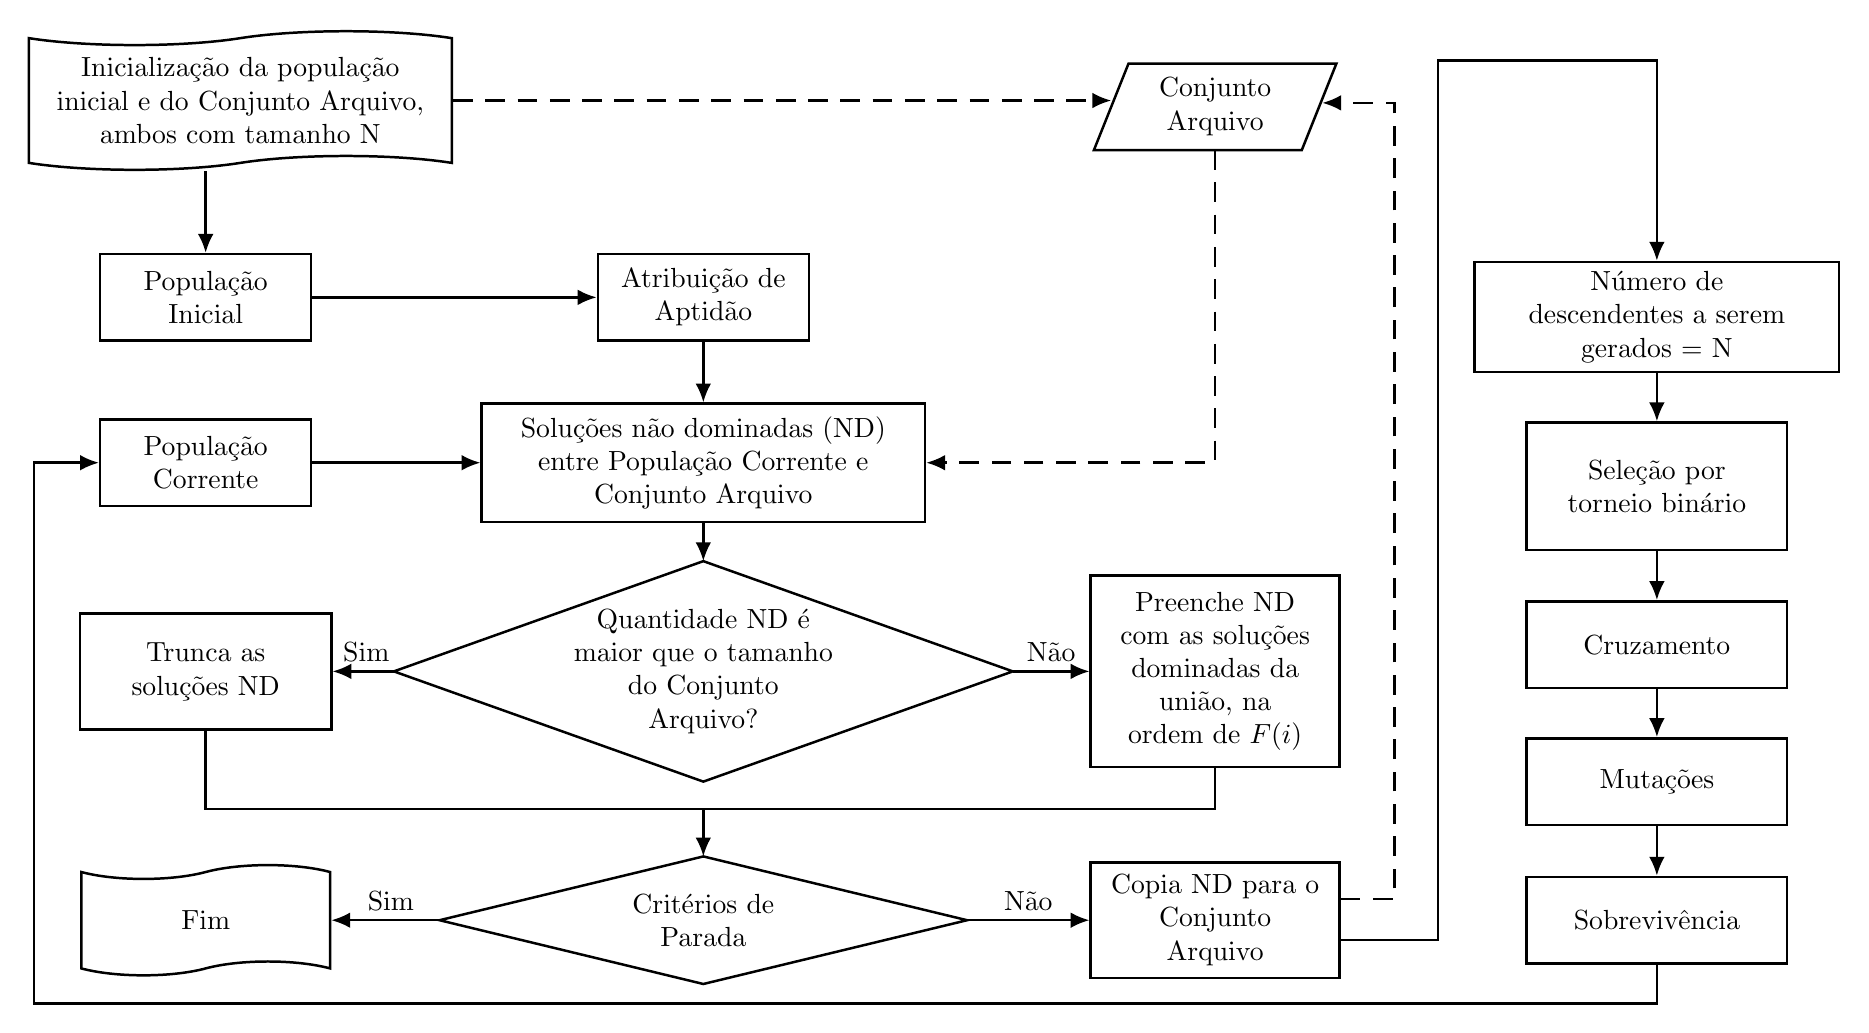
\begin{tikzpicture}[
    line width=0.9pt,
    >={Latex[length=2.4mm,width=2mm]},
    box/.style={draw, align=center, inner sep=1pt},
    tracejado/.style={dash pattern=on 2.5mm off 1.6mm},
    rotulo/.style={inner sep=1pt, anchor=south},
  ]

  % Caixas
  \node[draw, tape, align=center, minimum width=5.37cm, minimum height=1.76cm]
    (init) at (2.69,-1.10) {Inicialização da população\\inicial e do Conjunto Arquivo,\\ambos com tamanho N};
  \draw (13.97,-0.63) -- (16.61,-0.63) -- (16.17,-1.73) -- (13.53,-1.73) -- cycle;
  \node[align=center] (arq) at (15.07,-1.18) {Conjunto\\Arquivo};

  \node[box, minimum width=4.63cm, minimum height=1.40cm] (ndesc) at (20.68,-3.85)
    {Número de\\descendentes a serem\\gerados = N};
  \node[box, minimum width=2.68cm, minimum height=1.10cm] (popini) at (2.25,-3.60) {População\\Inicial};
  \node[box, minimum width=2.68cm, minimum height=1.10cm] (aptid) at (8.57,-3.60) {Atribuição de\\Aptidão};
  \node[box, minimum width=2.68cm, minimum height=1.10cm] (popcor) at (2.25,-5.70) {População\\Corrente};
  \node[box, minimum width=5.63cm, minimum height=1.50cm] (nd) at (8.57,-5.70)
    {Soluções não dominadas (ND)\\entre População Corrente e\\Conjunto Arquivo};
  \node[box, minimum width=3.31cm, minimum height=1.62cm] (torneio) at (20.68,-6.00) {Seleção por\\torneio binário};

  \draw (8.57,-6.95) -- (12.50,-8.35) -- (8.57,-9.75) -- (4.64,-8.35) -- cycle;
  \node[align=center] at (8.57,-8.35) {Quantidade ND é\\maior que o tamanho\\do Conjunto\\Arquivo?};
  \node[box, minimum width=3.19cm, minimum height=1.47cm] (trunca) at (2.25,-8.35) {Trunca as\\soluções ND};
  \node[box, minimum width=3.16cm, minimum height=2.43cm] (preenche) at (15.07,-8.35)
    {Preenche ND\\com as soluções\\dominadas da\\união, na\\ordem de $F(i)$};
  \node[box, minimum width=3.31cm, minimum height=1.10cm] (cruz) at (20.68,-8.01) {Cruzamento};
  \node[box, minimum width=3.31cm, minimum height=1.10cm] (mut) at (20.68,-9.75) {Mutações};

  \draw (8.57,-10.70) -- (11.92,-11.51) -- (8.57,-12.32) -- (5.22,-11.51) -- cycle;
  \node[align=center] at (8.57,-11.51) {Critérios de\\Parada};
  \node[draw, tape, align=center, minimum width=3.16cm, minimum height=1.40cm] (fim) at (2.25,-11.51) {Fim};
  \node[box, minimum width=3.16cm, minimum height=1.47cm] (copia) at (15.07,-11.51)
    {Copia ND para o\\Conjunto\\Arquivo};
  \node[box, minimum width=3.31cm, minimum height=1.10cm] (sobrev) at (20.68,-11.51) {Sobrevivência};

  % Fluxo principal
  \draw[->] (2.25,-2.00) -- (popini.north);
  \draw[->] (popini.east) -- (aptid.west);
  \draw[->] (aptid.south) -- (nd.north);
  \draw[->] (popcor.east) -- (nd.west);
  \draw[->] (nd.south) -- (8.57,-6.95);

  \draw[->] (4.64,-8.35) -- (trunca.east) node[rotulo, pos=0.45, yshift=2pt] {Sim};
  \draw[->] (12.50,-8.35) -- (preenche.west) node[rotulo, pos=0.5, yshift=2pt] {Não};
  \draw (trunca.south) -- (2.25,-10.10) -- (15.07,-10.10) -- (preenche.south);
  \draw[->] (8.57,-10.10) -- (8.57,-10.70);

  \draw[->] (5.22,-11.51) -- (fim.east) node[rotulo, pos=0.45, yshift=2pt] {Sim};
  \draw[->] (11.92,-11.51) -- (copia.west) node[rotulo, pos=0.5, yshift=2pt] {Não};

  % Conjunto arquivo (tracejado)
  \draw[->, tracejado] (init.east) -- (13.75,-1.10);
  \draw[->, tracejado] (15.07,-1.73) -- (15.07,-5.70) -- (nd.east);
  \draw[->, tracejado] (copia.east |- 0,-11.24) -- (17.35,-11.24) -- (17.35,-1.13) -- (16.43,-1.13);

  % Reprodução
  \draw[->] (copia.east |- 0,-11.76) -- (17.90,-11.76) -- (17.90,-0.59) -- (20.68,-0.59) -- (ndesc.north);
  \draw[->] (ndesc.south) -- (torneio.north);
  \draw[->] (torneio.south) -- (cruz.north);
  \draw[->] (cruz.south) -- (mut.north);
  \draw[->] (mut.south) -- (sobrev.north);
  \draw[->] (sobrev.south) -- (20.68,-12.57) -- (0.07,-12.57) -- (0.07,-5.70) -- (popcor.west);
\end{tikzpicture}
\end{document}
